\documentclass[12pt]{article}

\usepackage[utf8]{inputenc}
\usepackage[T1]{fontenc}
\usepackage{geometry}
\usepackage{graphicx} %figures
\usepackage{subfig} %subfigures
\usepackage{gensymb} %degree sign
\usepackage{amsmath} %math stuff
\usepackage{bm} %bold stuff
\usepackage[]{algorithm2e} %algorithms
\geometry{a4paper}

\title{\textbf{Part 7: Trust Region Optimization}}

\begin{document}
\date{January 18, 2021}
\maketitle

Hey everyone! Today's post will go over something that we have discussed in some detail before: optimization! Specifically, Trust-Region methods for convex optimization. For this we will by happenstance go over Gauss Newton method as well. First let's do the easiest version of gradient based optimization: Gradient Descent. We start with the \emph{Update Rule}: $x_{k+1}=x_k+g$ where in the case of Gradient Descent:

\begin{align*}
g=-\alpha\nabla f(x_k)
\end{align*}

\vspace{5mm}

The descent direction $g$ is equal to the gradient at the point $x_k$.

\vspace{5mm}

\begin{algorithm}[H]
Initialize $x_0, \: \alpha>0$\;
\For{$k = 1:K$}{
$x_{k+1}=x_k+\alpha g$\;}
 \caption{General Descent Method}
\end{algorithm}

\vspace{5mm}

Note that $\alpha$ (step size) is a constant that modulates the size of the difference between $x_{k+1}$ and $x_k$. Also note that $-1$ is multiplied by $g$ so that when $g>0$ (i.e. we go up) Gradient Descent moves in the opposite direction.

\section{Newton/Gauss-Newton Method}

Next we will talk about the Newton method, which is similar to Gradient Descent but utilizes Hessian $\nabla^2 f(x)$ information:

\begin{align*}
g=-\nabla^2 f(x_k)^{-1} \nabla f(x_k)
\end{align*}

\vspace{5mm}

This leads to the beloved Quasi-Newton methods where $B_k \approx \nabla^2 f(x_k)$ because the Hessian is often difficult to calculate. A modification of Newton's method is Gauss-Newton's method where:

\begin{align*}
g= (\nabla f(x_k) \nabla^T f(x_k))^{-1} \nabla f(x_k) f(x)
\end{align*}

\section{Trust Region Concept}

The basic idea behind Trust Regions is that we optimize a function in a small space where we have a good approximation of the surface $f(x)$ through a Taylor Series approximation $m$ around $x$ plus some vector $p$ for gradient $g$ and Hessian approximation $B$. 

\vspace{5mm}

\begin{align*}
f(x+p) \approx m(p)=f_k+g_k+1/2g_k^TB_kp_k
\end{align*}

\vspace{5mm}

We solve the problem:

\begin{align*}
p^*=argmin m(p) \: \text{s.t.} \: ||p|| \leq \delta_k
\end{align*}

\vspace{5mm}

Which basically means minimize $m$ approximation of $f(x)$ for some distance $p$ constrained on the ball of radius $\delta_k$ (using the $L2$ norm). The simplest solution to this problem is the Full Step: 

\begin{equation}
p_{B}=-B_k^{-1}g_k
\end{equation}

\vspace{5mm}

Which is optimal when (i) $B_k$ is PD and (ii) $||B_k^{-1}g_k||<=\delta_k$, which is the unconstrained minimization of $m(p)$. 

\section{Trust Region Algorithm}

We define an improvement metric:

\vspace{5mm}

\begin{align*}
\rho_k=\dfrac{f(x_k)-f(x_k+p_k)}{m_k(0)-m_k(p_k)}
\end{align*}

\vspace{5mm}

Which is the ratio of the reduction in $f(x_k)$ to the approximation in $m(p_k)$. The closer to $\rho_k=1$ the better. The Trust Region algorithm incorporates this calculation as follows:

\vspace{5mm}

\begin{algorithm}[H]
Initialize $\hat{\Delta}>0 \: \Delta_o \in (0,\hat{\Delta}) \: \eta \in [0,1/4)$ \;
\For{$k = 1:K$}{
Calculate $p_k$ \; 
Calculate $\rho_k$ \;
\uIf{$\rho_k<1/4$}{
$\Delta_{k+1}=1/2 \Delta_k$ \;}
\uElse{
\uIf{$\rho_k>3/4 \: ||p_k||=\Delta_k$}{$\Delta_k=min \{2\Delta_k,\hat{\Delta}\}$}
\uElse{$\Delta_k=\hat{\Delta}$}}
\uIf{$\rho_k>\eta$}{$x_{k+1}=x_k+p_k$}
\uElse{$x_{k+1}=x_k$}
}
\caption{General Trust Region Method}
\end{algorithm}

\vspace{5mm}

What we need to do is basically solve for $p_k$ and adjust $\Delta_k$.

\subsection{Cauchy Point}

The next most basic solution to the subproblem in the Trust Region algorithm is the Cauchy Point. 

\begin{align*}
\tau_k=
\begin{cases}
    1 & \text{if } \: g_k^T B_k g_k \leq 0\\
    min\{||g_k||^3/(\Delta_k g^T_k B_k g_k),1\} & \text{otherwise}
\end{cases}
\end{align*}

\begin{equation}
p_c=-\dfrac{\tau_k \Delta_k g_k}{||g_k||}
\end{equation}

Think about the Cauchy Point as $p$ which gives the steepest descent subject the the constraint talked about above. One way to implement the Cauchy Point is to use $p_B$ when $B_k$ is PD and $||p_B||<\Delta_k$, and $p_c$ elsewhere.

\subsection{Dogleg Method}

This one took a while to implement but here we go. Specifically we implement the Dogleg Method from Powell's Numerical Optimization Book, which tends to be useful when $B_k$ is PD (but don't take my word for it). After we calculate $\tau$, $p_u$ (steepest descent direction) and $p_B$ (full step solution) we can use the following:

\vspace{5mm}

\begin{equation}
p_k=
\begin{cases}
    \tau p_u & \text{if } \: 0 \leq \tau \leq 1\\
    p_u+(\tau-1)(p_B-p_u) & \text{if} \: 1 \leq \tau \leq 2
\end{cases}
\end{equation}

\section{Example Problem}

Here we throw some of these methods at the modified 2-D Himmelblau problem:

\begin{align*}
f(x) = (x_1^2 + x_2 - 11)^2 + (x_1 + x_2^2 - 7)^2
\end{align*}

\begin{figure}[h]
\centering
\subfloat[][$f(x)$]{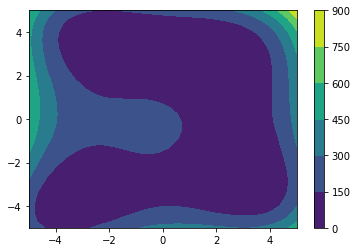
\includegraphics[width=0.4\textwidth]{Post_7_himmel1}}
\subfloat[][Locations of non-PD]{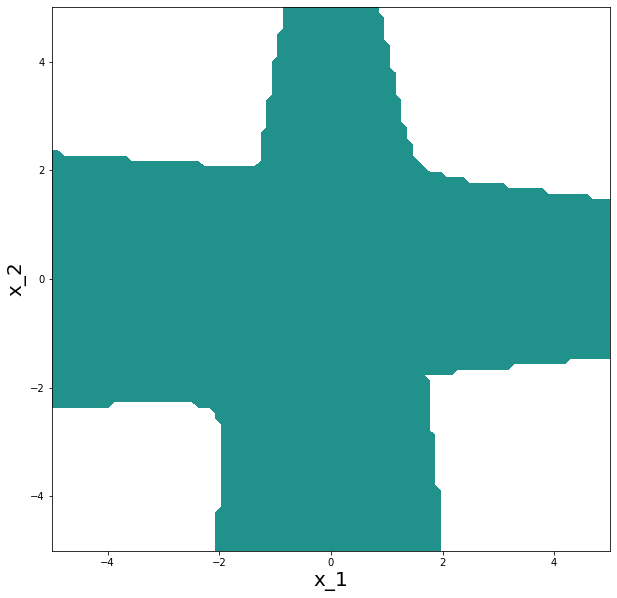
\includegraphics[width=0.3\textwidth]{Post_7_himmel2}}
\caption{Himmelblau Function}
\end{figure}

\vspace{5mm}

Here we do six random initializations of some of the methods we have talked about.

\vspace{5mm}

\begin{figure}[h]
\centering
\subfloat[][]{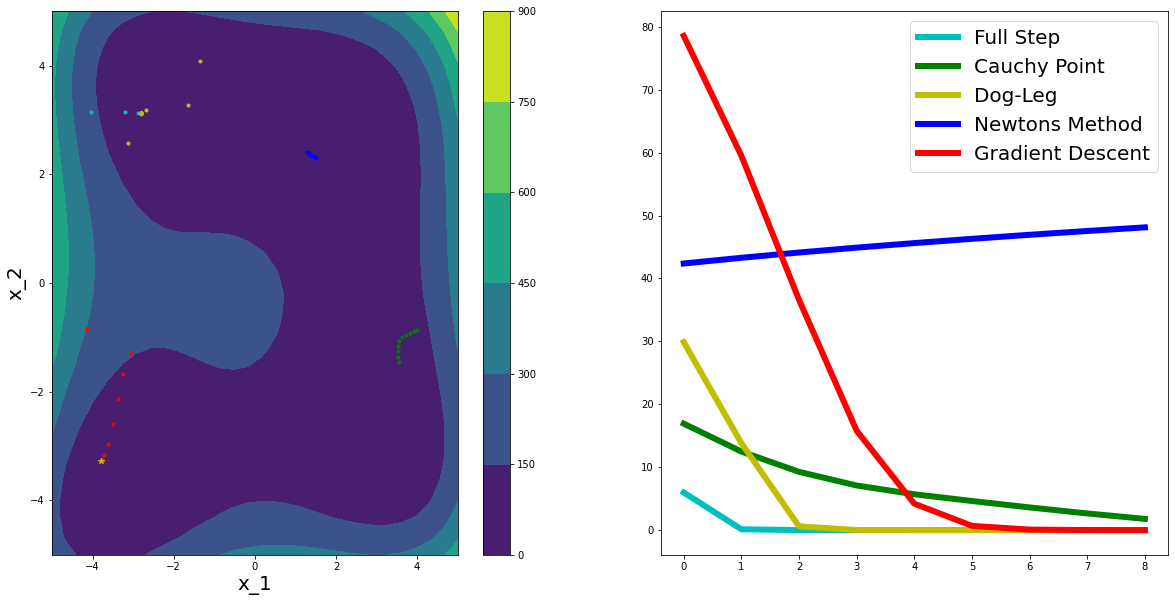
\includegraphics[width=0.45\textwidth]{Post_7_opt1}}
\subfloat[][]{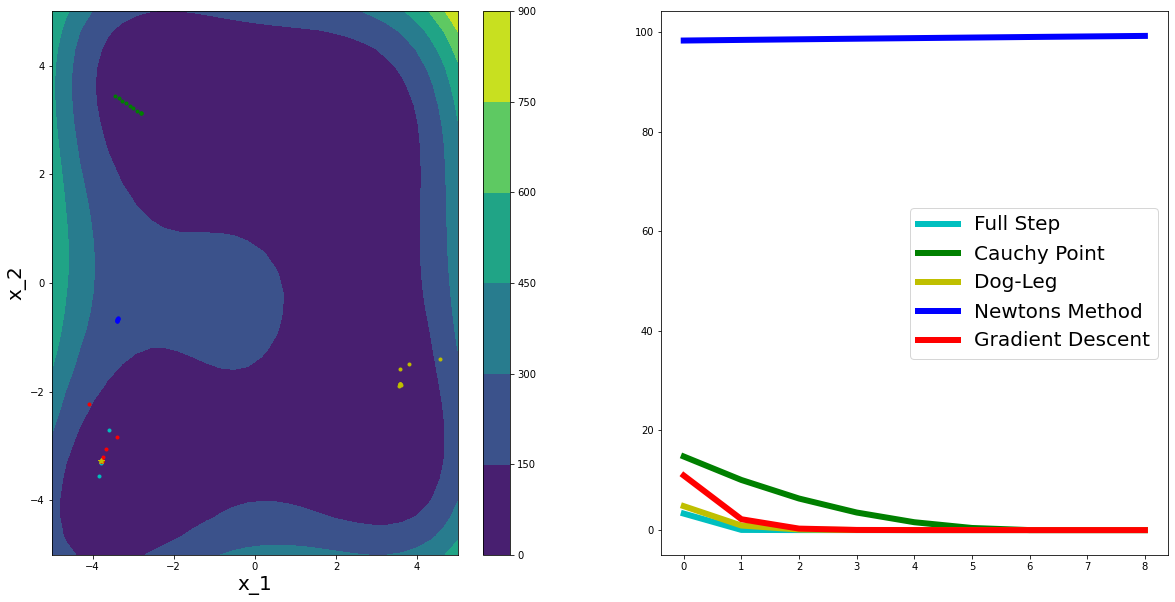
\includegraphics[width=0.45\textwidth]{Post_7_opt2}}

\subfloat[][]{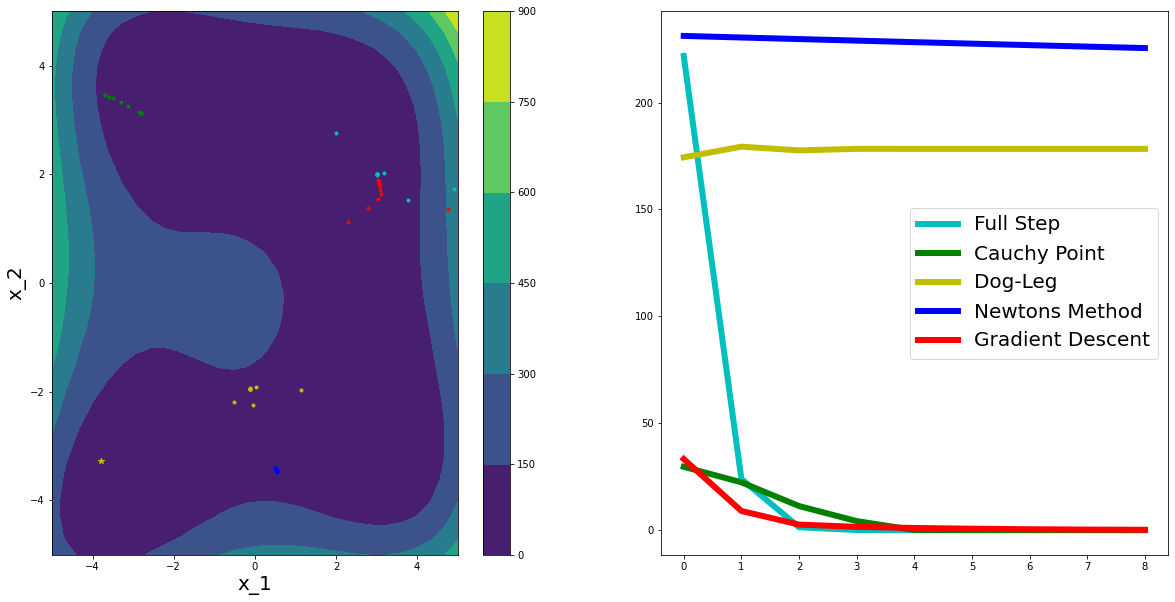
\includegraphics[width=0.45\textwidth]{Post_7_opt3}}
\subfloat[][]{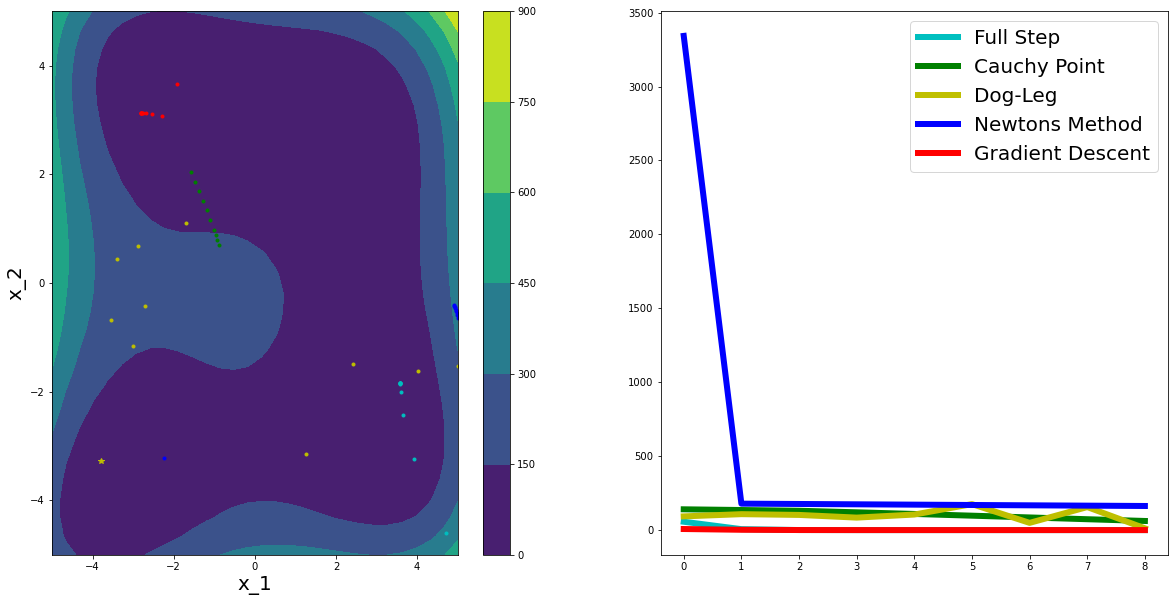
\includegraphics[width=0.45\textwidth]{Post_7_opt4}}

\subfloat[][]{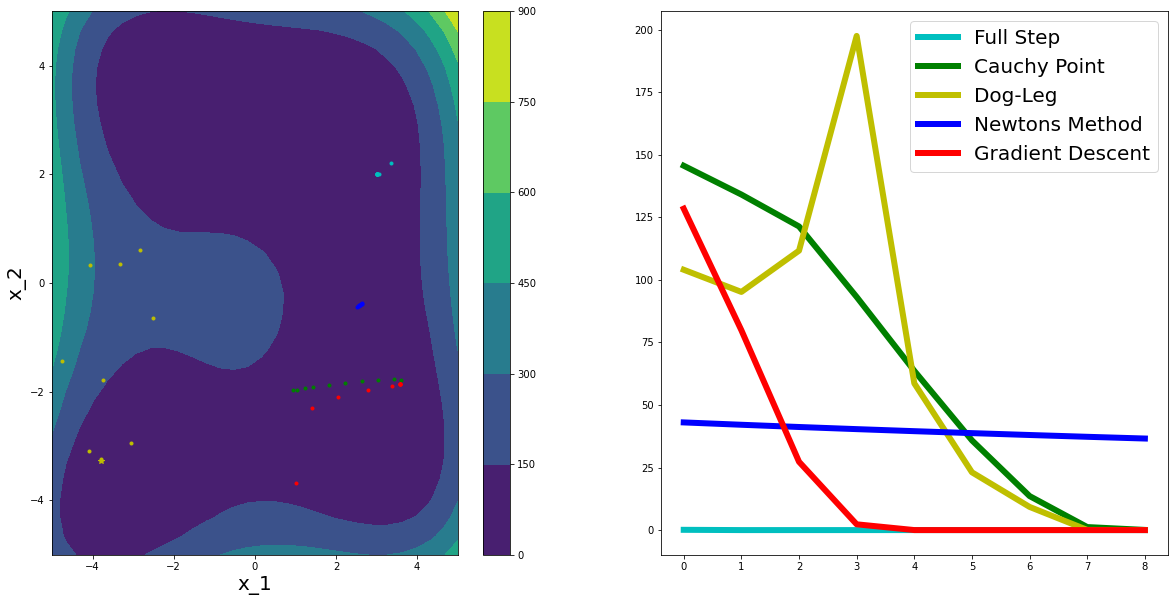
\includegraphics[width=0.45\textwidth]{Post_7_opt5}}
\subfloat[][]{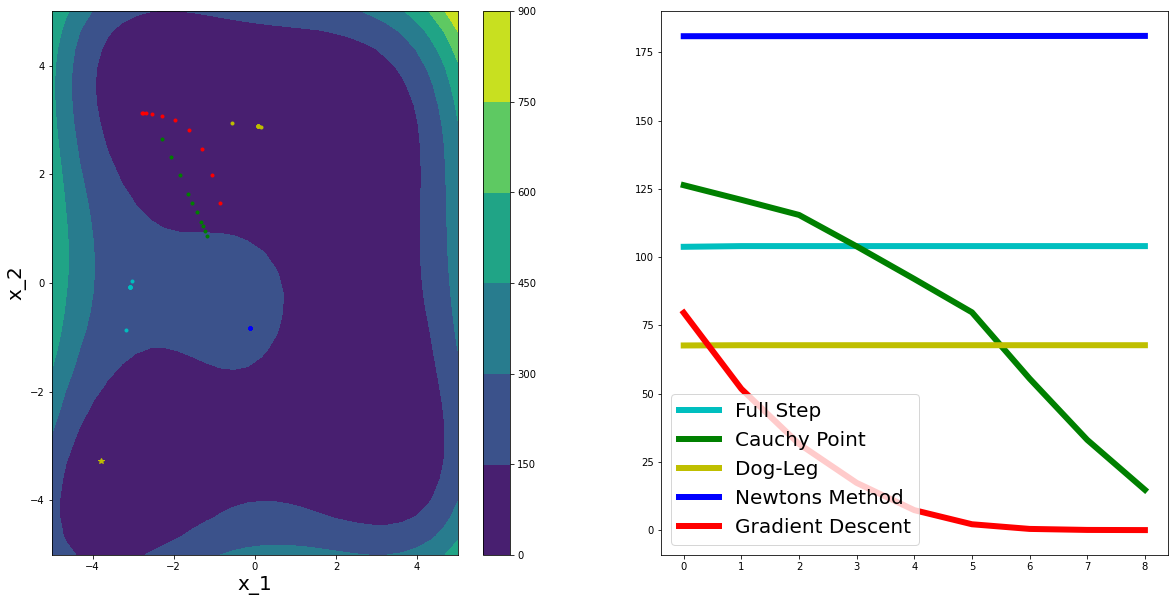
\includegraphics[width=0.45\textwidth]{Post_7_opt6}}
\caption{Example Optimization Problem | $\eta=0.1$, $\hat{\Delta}=1$}
\end{figure}

\vspace{5mm}

This is a very difficult optimization problem to solve and we did an okay job. In theory we should be taking a look at the positive definiteness of the region we are in and select the method based on that (which is what more sophisticated methods do). Great job everyone! I am not sure what I will present next week so I'll just say we'll do something related to BOTorch.

\end{document}